%%
%% This is file `sample-sigconf.tex',
%% generated with the docstrip utility.
%%
%% The original source files were:
%%
%% samples.dtx  (with options: `sigconf')
%% 
%% IMPORTANT NOTICE:
%% 
%% For the copyright see the source file.
%% 
%% Any modified versions of this file must be renamed
%% with new filenames distinct from sample-sigconf.tex.
%% 
%% For distribution of the original source see the terms
%% for copying and modification in the file samples.dtx.
%% 
%% This generated file may be distributed as long as the
%% original source files, as listed above, are part of the
%% same distribution. (The sources need not necessarily be
%% in the same archive or directory.)
%%
%% The first command in your LaTeX source must be the \documentclass command.
\documentclass[sigconf,nonacm=true]{acmart}
\usepackage{listings}
\usepackage{booktabs}% More proffesional look of tables.
\usepackage{siunitx}% An awesome package for typesetting and manipulation numbers and units.
\usepackage{caption}% Better control over caption
\usepackage{lipsum}% Example text
\usepackage{xcolor}
\usepackage{adjustbox}
\usepackage{booktabs}

\lstset{
	basicstyle=\ttfamily,
	columns=fullflexible,
	frame=single,
	breaklines=true,
	postbreak=\mbox{\textcolor{red}{$\hookrightarrow$}\space},
}

\pagecolor{white}
\lstset{
basicstyle=\ttfamily,
frame=single
}
%%
%% \BibTeX command to typeset BibTeX logo in the docs
\AtBeginDocument{%
  \providecommand\BibTeX{{%
    \normalfont B\kern-0.5em{\scshape i\kern-0.25em b}\kern-0.8em\TeX}}}

%% Rights management information.  This information is sent to you
%% when you complete the rights form.  These commands have SAMPLE
%% values in them; it is your responsibility as an author to replace
%% the commands and values with those provided to you when you
%% complete the rights form.
\setcopyright{none}
%%\copyrightyear{2020}
%%\acmYear{2020}
%%\acmDOI{10.1145/1122445.1122456}

%% These commands are for a PROCEEDINGS abstract or paper.
%% \acmConference[Woodstock '18]{Woodstock '18: ACM Symposium on Neural
%%   Gaze Detection}{June 03--05, 2018}{Woodstock, NY}
%% \acmBooktitle{Woodstock '18: ACM Symposium on Neural Gaze Detection,
%%   June 03--05, 2018, Woodstock, NY}
%% \acmPrice{15.00}
%% \acmISBN{978-1-4503-XXXX-X/18/06}


%%
%% Submission ID.
%% Use this when submitting an article to a sponsored event. You'll
%% receive a unique submission ID from the organizers
%% of the event, and this ID should be used as the parameter to this command.
%%\acmSubmissionID{123-A56-BU3}

%%
%% The majority of ACM publications use numbered citations and
%% references.  The command \citestyle{authoryear} switches to the
%% "author year" style.
%%
%% If you are preparing content for an event
%% sponsored by ACM SIGGRAPH, you must use the "author year" style of
%% citations and references.
%% Uncommenting
%% the next command will enable that style.
%%\citestyle{acmauthoryear}

%%
%% end of the preamble, start of the body of the document source.
\begin{document}

%%
%% The "title" command has an optional parameter,
%% allowing the author to define a "short title" to be used in page headers.
\title{CE/CZ4045 Assignment Part 2}

%%
%% The "author" command and its associated commands are used to define
%% the authors and their affiliations.
%% Of note is the shared affiliation of the first two authors, and the
%% "authornote" and "authornotemark" commands
%% used to denote shared contribution to the research.

\author{Lim Jun Hong}
\affiliation{\institution{Nanyang Technological University}}
\email{LIMJ0209@e.ntu.edu.sg}

\author{Tammy Lim Lee Xin}
\affiliation{\institution{Nanyang Technological University}}
\email{TLIM045@e.ntu.edu.sg}

\author{Lee Han Wei}
\affiliation{\institution{Nanyang Technological University}}
\email{B160017@e.ntu.edu.sg}

\author{Pang Yu Shao}
\affiliation{\institution{Nanyang Technological University}}
\email{C170134@e.ntu.edu.sg}

%%
%% By default, the full list of authors will be used in the page
%% headers. Often, this list is too long, and will overlap
%% other information printed in the page headers. This command allows
%% the author to define a more concise list
%% of authors' names for this purpose.
%% \renewcommand{\shortauthors}{Trovato and Tobin, et al.}

%%
%% The abstract is a short summary of the work to be presented in the
%% article.
%%\begin{abstract}
%%  TODO:
%%\end{abstract}



%%
%% Keywords. The author(s) should pick words that accurately describe
%% the work being presented. Separate the keywords with commas.
%% \keywords{Deep Learning, NLP, Neural Networks}

%% A "teaser" image appears between the author and affiliation
%% information and the body of the document, and typically spans the
%% page.

%% \begin{teaserfigure}
%%   \includegraphics[width=\textwidth]{sampleteaser}
%%   \caption{Seattle Mariners at Spring Training, 2010.}
%%   \Description{Enjoying the baseball game from the third-base
%%   seats. Ichiro Suzuki preparing to bat.}
%%   \label{fig:teaser}
%% \end{teaserfigure}

%%
%% This command processes the author and affiliation and title
%% information and builds the first part of the formatted document.
\maketitle

\section{Introduction}
For this assignment, we implement two different Neural Network models using \verb|Pytorch| to perform NLP tasks such as \textbf{Text Prediction/ Generation} as well as \textbf{Named Entity Recognition (NER)}

\section{Designing a Feed-Forward Neural Network for Text Generation}
In this section, a simple Feed-Forward Neural Network (FFN) architecture
will be designed and implemented for the purpose of language modelling
(i.e., to predict the next word given a sequence of words.)

\subsection{Dataset}
\label{subsection:dataset}
The dataset to be used for this task is the \textbf{wikitext-2} dataset,
which is a collection of text from Wikipedia.
\subsubsection{Data Pre-processing}
Various pre-processing is done to the dataset before it is used to train the 
model, such as:

\textbf{Case-folding} (i.e., reducing all alphabet characters to lower case): 
This is done as same words with different characters in differing cases are
treated as separate words. For instance, \verb|"The"| and \verb|"the"| would
be treated as 2 completely different words and would be mapped to different 
Word IDs, which may result in completely different embeddings.

\textbf{Removal of headings}: Upon inspection of the dataset, many lines containing
section headings can be identified. An example of a heading is given below:

\verb| = = = Influence on Japanese literature = = = |

Therefore, such lines shall be discarded to prevent our model from learning 
and predicting the header tokens \verb|"="|.


\subsection{Implementing the Baseline FFN}

Refer to Figure ~\ref{fig:ffnarch} for the architecture of the proposed FFN.

\begin{figure*}
	\centering
	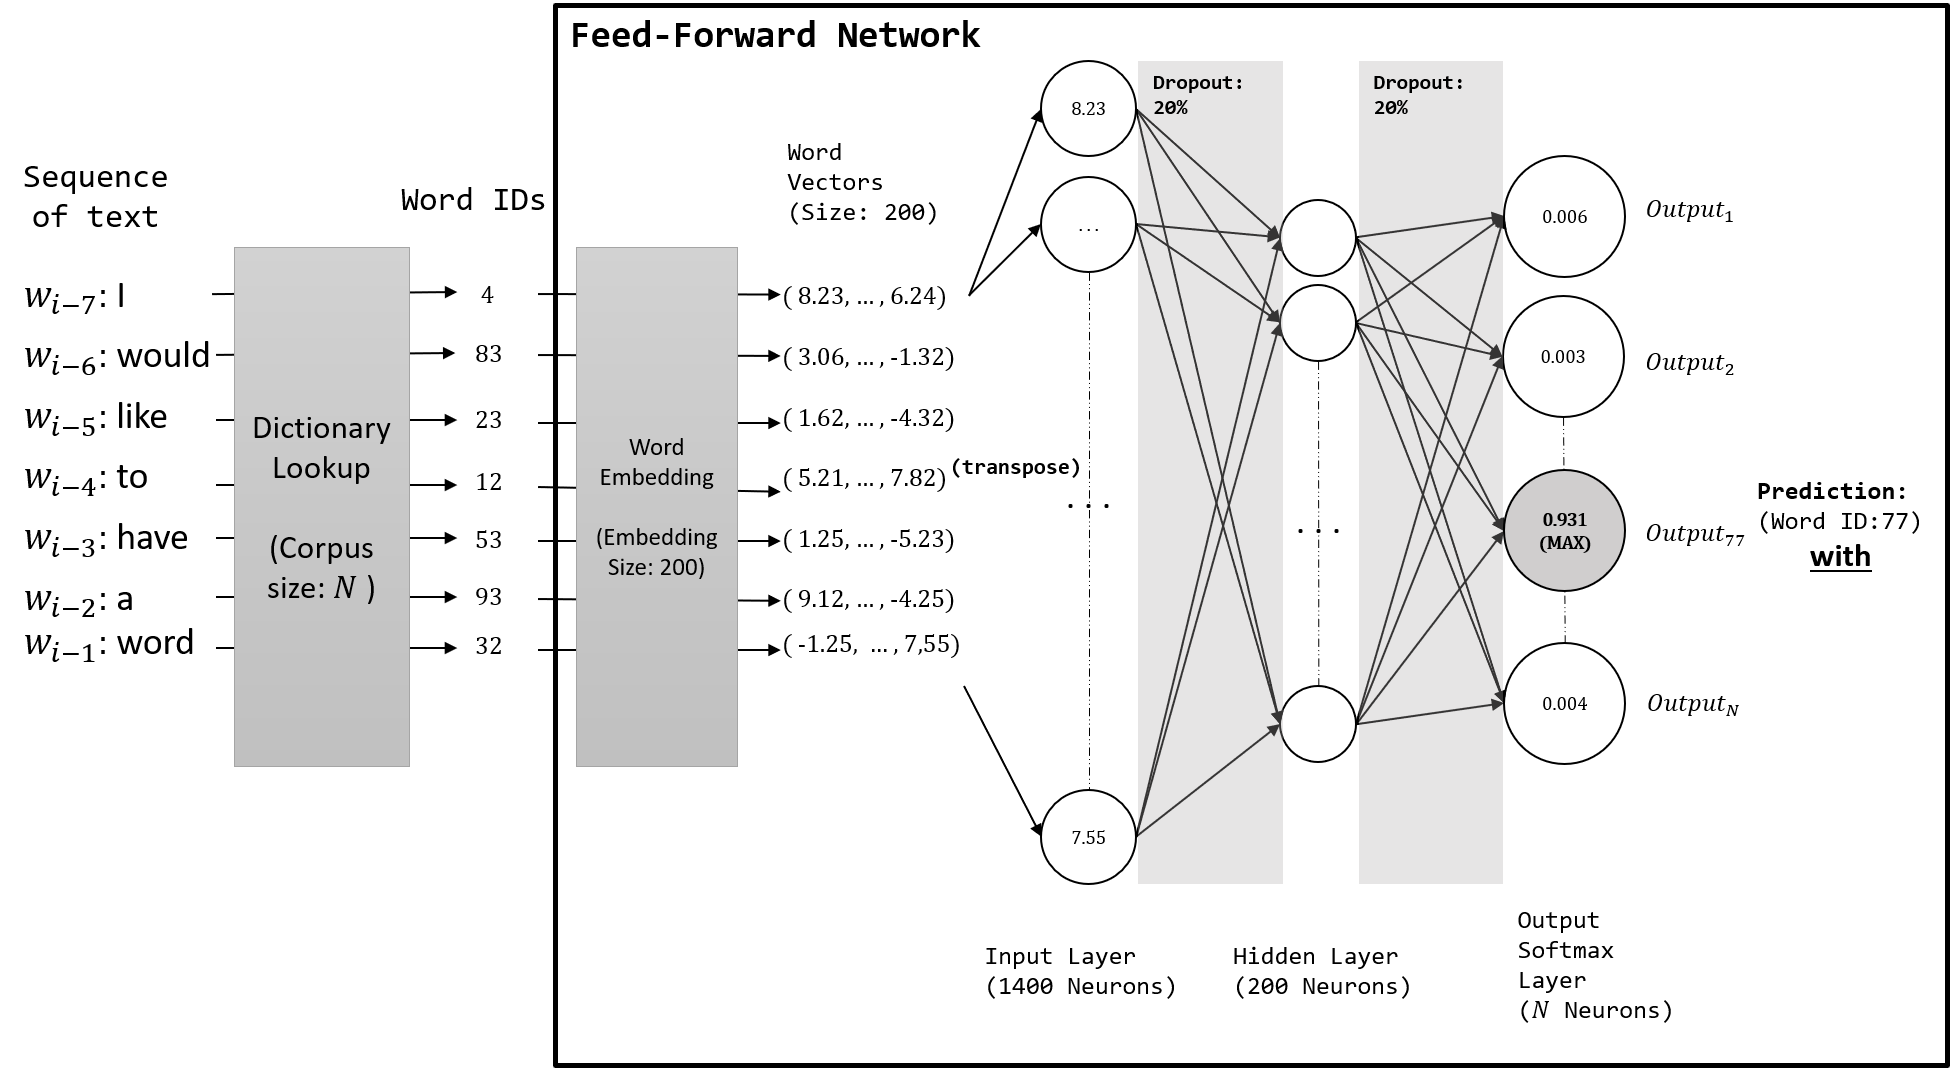
\includegraphics[scale=0.52]{figures/ffn.png}
	\caption{Architecture of FFN}
	\label{fig:ffnarch}
	
\end{figure*}


\subsubsection{Input Layer}
As the model is to be trained on 8-grams (i.e., a sequence of 8 words),
the input to the FFN will be the first 7 words (in word IDs format). The
input layer will then convert the word IDs to its word vectors.
These word vectors will be transposed and "concatenated" and fed as 
inputs to the hidden layer.

\subsubsection{Hidden Layer}
The hidden layer of the network is a simple dense layer of 
\textbf{200 neurons} in the beginning and will be tuned for further gains 
in subsequent sections. The activation function used for the hidden layer 
is the \textbf{tanh} function before the outputs are fed to the output layer.

\subsubsection{Output Layer}
The output layer of the network is a \textbf{Softmax} layer which gives 
the probability of the word ID representing the predicted word following 
the sequence of 7 preceding words that are fed into the input layer.

\subsubsection{Training Set-up and Hyperparameters} \label{subsubsection:baselinesetup}
For the baseline model, the following set-up and hyperparameters are used:
\begin{itemize}
	\item Learning Rate: \textbf{0.0001} (With annealing factor of \textbf{0.25})
	\item Optimiser: \textbf{Adam}
	\item Hidden Layers: \textbf{1}
	\item Neurons in Hidden Layers: \textbf{200}
	\item Dropout in each layer: \textbf{20\%}
	\item Training Epochs: \textbf{50}
	\item Loss function: \textbf{Cross-Entropy}
\end{itemize}

\subsection{Training Results of the Baseline FFN}
\label{subsection:baselineresults}
After training the FFN for 50 epochs with the set-up described in 
\ref{subsubsection:baselinesetup}, the "best" results are obtained at the epoch
with the lowest validation loss:  

\begin{table}[H]
	\label{tab:freq}
	\begin{adjustbox}{width=\columnwidth}
	\begin{tabular}{cccc}
		\toprule
		Epoch: 20&Loss (Cross-Entropy)&Perplexity&Prediction Accuracy\\
		\midrule
		Training Set & 4.86 & 128.79 & 26.4\% \\
		Validation Set & 5.40 & 221.29 & 20.6\% \\
		\bottomrule
	\end{tabular}
	\end{adjustbox}
	\caption{Best Baseline FFN Training Results}
\end{table}

\begin{figure}[H]
	\centering
	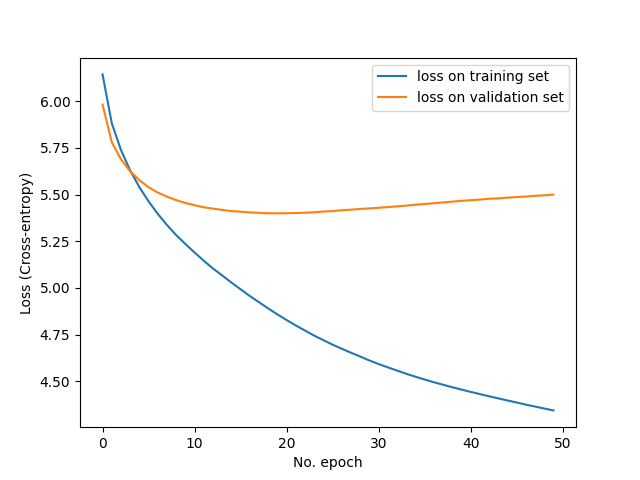
\includegraphics[scale=0.47]{figures/baseline_adam_loss.png}
	\caption{Loss of Baseline Model Over 50 Epochs}
	\label{fig:baseloss}
\end{figure}

\subsubsection{Analysis}
From the obtained results, it can be seen that from Figure \ref{fig:baseloss} there is heavy over-fitting of the model from about 
epoch 20 onwards. The performance of the model in terms of prediction 
accuracy on the validation set is only at \textbf{20.6\%} and a perplexity score of \textbf{221.29} at epoch 20.

In the following sections, we will aim to improve on this Baseline FFN's accuracy
by experimenting with various strategies such as
\textbf{Regularisation} as well as \textbf{Hyperparameter tuning} to arrive at a
model with the best performance.

\subsection{Overcoming Over-fitting}
\textbf{Over-fitting} occurs when a model learns the training data too closely, and as a result, fails to \textbf{generalise} to unseen data. This is clearly seen in Figure \ref{fig:baseloss} where the model's loss on training data is shown to continue decreasing while the model's loss on the validation data is shown to be increasing. This means that while the model would perform very well when predicting inputs from the training set, it would not perform well for the prediction of unseen input data.

\subsubsection{Early Stopping}
\textbf{Early stopping}, as its name implies, is a technique used to halt training of the model prematurely when over-fitting is detected. While it does not ensure that overfitting is reduced and the model would have a better performance, it will ensure that the model would not be over-trained. This would therefore save time that would be otherwise spent on training the model. For the training of the model in Section \ref{subsection:baselineresults}, Early Stopping would stop the training shortly after Epoch 20 as the validation loss did not improve after that.

For subsequent models, Early Stopping will be implemented with a \textbf{patience} of 5 Epochs. This means that if the \textbf{validation loss} does not improve for 5 consecutive Epochs, the training would be halted prematurely.

\subsubsection{L2 Regularisation}
\textbf{L2 Regularisation} is one of the strategies that can be used to prevent over-fitting of a model. One of the causes of over-fitting is when there are very high weight values learnt by the model which causes a the model to learn one feature very closely/strongly which may only be specific to the training data. 

Therefore, L2 Regularisation aims to prevent over-fitting of the model by penalizing very large weights that are learned by the model. This is done by summing all the squared weight values and then multiplying them by a factor before adding it to the computed error value. This results in the following loss function:
\begin{equation}\label{key}
Loss = Error + \beta\sum_{i=1}^{W}{W_{i}}^{2}
\end{equation}
Where Error is the Cross-Entropy loss and \(\mathbf{\beta}\) is the regularising factor.

A L2 regularisation factor of \(\mathbf{10^{-6}}\) is applied and implemented in Pytorch as a \textbf{weight decay} parameter to the optimiser. As a result, the training took longer to converge. The training was done for \textbf{100} epochs instead of 50 to allow the model more time to converge. 

During the training process, the model did not detect over-fitting and hence did not terminate early. At the end of the 100 epochs, the model had considerably better performance on the validation set as compared to the initial baseline model.

\begin{table}[H]
	\label{tab:regbasecomp}
	\begin{adjustbox}{width=\columnwidth}
		\begin{tabular}{cccc}
			\toprule
			&\multicolumn{3}{c}{(Metrics evaluated on \textbf{Validation} Set)}\\
			Model &Best Perplexity&Best Loss&Best Prediction Accuracy\\
			\midrule
			Baseline & 221.29 & 5.40 & 20.6\% \\
			With L2 Reg & 183.53 & 5.21 & 21.5\% \\
			\midrule
			$\Delta$Perplexity Score & \textbf{-37.76}\\
			\bottomrule
		\end{tabular}
	\end{adjustbox}
	\caption{Performance of model with L2 Regularisation}
\end{table}

\begin{figure}[H]
	\centering
	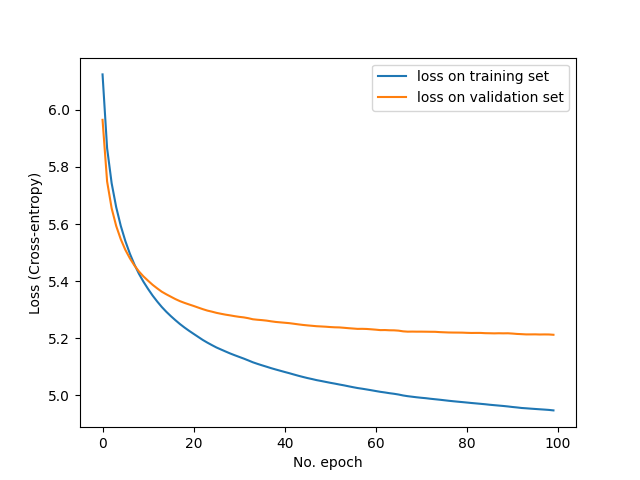
\includegraphics[scale=0.47]{figures/l2_loss.png}
	\caption{Loss of Model with L2 Over 100 Epochs}
	\label{fig:l2loss}
\end{figure}


\subsection{Hyperparameter Tuning}
With the over-fitting measures in place, this sub-section aims to further improve on the model's performance by tuning the hyperparameters of the model. Specifically, the effects of tuning the  \textbf{Embedding Size} and \textbf{Hidden Layer Size} of the network will be evaluated and hyperparameters yielding the best performing will be chosen.
\subsubsection{Methodology}
A simple \textbf{Grid Search} is performed on the two hyperparameters. The Embedding Size and Hidden Layer Size are also kept to the same to each other as it is required to explore the effects of \textbf{Parameter Sharing} in a later section. The following values are used for the Grid Search:

\begin{displaymath}
Size \in \{200, 300, 400, 500, 600, 700, 800\}
\end{displaymath}
\subsubsection{Results} 
The grid search was performed and the following results are obtained:
\begin{table}[h]
\label{tab:gridsearch}
	\begin{adjustbox}{width=\columnwidth}
		\begin{tabular}{cccccccc}
			\toprule
			Emb Size \& nhid Size & 200 & 300 & \textbf{400} & 500 & 600 & 700 & 800 \\
			\midrule
			Validation Perplexity& 183.53 & 179.75 & \textbf{179.45} & 180.40 & 181.76 & 182.99 & 184.38 \\
			\bottomrule
		\end{tabular}
	\end{adjustbox}

	\caption{Results of Grid Search}
\end{table}

From Table \ref{tab:gridsearch}, it can be seen that that an Embedding Size and Hidden Layer Size of \textbf{400} yields the best performance in terms of validation perplexity, therefore it is selected for the model.


\subsubsection{Further Refinements and Chosen Model}
\label{subsubsection:chosenmodel}
As the embedding and hidden layer dimensions have increased, the increased dimensions might lead to more over-fitting of the model. Therefore, the L2 regularisation term is increased from \(\mathbf{10^{-6}}\) to \(\mathbf{2 * 10^{-6}}\). 

The final specifications of the model are as follows:

\begin{itemize}
	\item Learning Rate: \textbf{0.0001} (With annealing factor of \textbf{0.25})
	\item Optimiser: \textbf{Adam}
	\item Embedding Size: \textbf{400}
	\item Hidden Layers: \textbf{1}
	\item Neurons in Hidden Layers: \textbf{400}
	\item Dropout in each layer: \textbf{20\%}
	\item L2 Regularisation Term: \(\mathbf{2 * 10^{-6}}\)

\end{itemize}

The model was trained for 95 Epochs, where it early-stopped when the validation loss ceased to decrease. The following results are obtained and compared with the baseline model:

\begin{table}[H]
	\label{tab:regbasecomp}
	\begin{adjustbox}{width=\columnwidth}
		\begin{tabular}{cccc}
			\toprule
			&\multicolumn{3}{c}{(Metrics evaluated on \textbf{Validation} Set)}\\
			Model &Best Perplexity&Best Loss&Best Prediction Accuracy\\
			\midrule
			Baseline & 221.29 & 5.40 & 20.6\% \\
			Final Model & 177.06 & 5.18 & 21.8\% \\
			\midrule
			$\Delta$Perplexity Score & \textbf{-44.23}\\
			\bottomrule
		\end{tabular}
	\end{adjustbox}
	\caption{Performance of Model w/ Hyperparameter Tuning}
\end{table}

\subsection{Parameter Sharing between Embedding and Output Softmax Layer}
In this section, the effects of Parameter Sharing (or \textbf{Weight Tying}) is explored. 

In previous studies, it is shown that sharing the parameters of the embeddings to the output softmax layer, would allow the output layer to have a more informed distribution than vanilla one-hot layers which would lead to improved learning. Also, the number of parameters to be learned by the model would also be reduced \cite{inan2016tying}, which could result in faster learning times per epoch.

\subsubsection{Results}
\label{subsubsection:weighttieresults}
With the model chosen in Section \ref{subsubsection:chosenmodel}, Parameter Sharing was implemented in Pytorch by simply assigning the encoder's weights to the decoder's weights
\begin{lstlisting}[language=Python]
self.decoder.weight = self.encoder.weight
\end{lstlisting}
The model is then trained until it early-stopped and the following observations are made:
\begin{itemize}
	\item The training reaches minimum validation loss at Epoch \textbf{85}, instead of \textbf{95} without weight tying.
	\item The time of training per Epoch is decreased from \textbf{67s} to \textbf{55s}
\end{itemize}
The following performance metrics are obtained:

\begin{table}[h]
	\begin{adjustbox}{width=\columnwidth}
		\begin{tabular}{cccc}
			\toprule
			&\multicolumn{3}{c}{(Metrics evaluated on \textbf{Validation} Set)}\\
			Model &Best Perplexity&Best Loss&Best Prediction Accuracy\\
			\midrule
			\textbf{Without} Weight Tying & 177.06 & 5.18 & 21.8\% \\
			\textbf{With} Weight Tying & 174.29 & 5.16 & 21.7\% \\
			\midrule
			$\Delta$Perplexity Score & \textbf{-2.77}\\
			\bottomrule
		\end{tabular}
	\end{adjustbox}
	\caption{Performance of Model w/ Parameter Sharing}
	\label{tab:weighttiecomp}
\end{table}

\subsubsection{Analysis}
With the observations made in Section \ref{subsubsection:weighttieresults} and Table \ref{tab:weighttiecomp}, it can be concluded that Parameter Sharing is indeed beneficial for language modelling. With Parameter Sharing, there are improvements in both having a final lower perplexity which indicates improved learning as well as having a faster training time of the model due to the decrease in the number of learnable parameters.


\subsection{Generating Words with Trained FNN Model}
To adapt \verb|generate.py| from Pytorch's example code to generate text with the implemented \verb|FNNModel|, there are two main steps that needs to be done.
\begin{itemize}
	\item Adapt the input to be 7 word IDs instead of 1 single word ID
	
	\begin{lstlisting}[language=python]
Before:
input = torch.randint(ntokens, (1, 1), dtype=torch.long).to(device)
After:
input = torch.randint(ntokens, (7, 1), dtype=torch.long).to(device)
	\end{lstlisting}
	
	\item With the generated output, append it to the end of the input tensor and remove the first word ID from the tensor.
	\begin{lstlisting}[language=python]
word_idx = torch.multinomial(word_weights, 1)[0]
word_tensor = torch.Tensor([[word_idx]]).long().to(device)
# Remove the first element using slicing
input = torch.cat([input[1:], word_tensor], 0)
word = corpus.dictionary.idx2word[word_idx]
	\end{lstlisting}
\end{itemize} 

\subsubsection{Results}
With the \verb|generate.py| implemented and working with the \verb|FNNModel|, it is then used to generate \textbf{200 words}. Refer to Appendix \ref{appendix:generated} for the full text generated.

\subsubsection{Analysis}
Upon inspection of the words generated by the model, one can see that it is mostly incoherent. However, there are some instances where the model seemed to perform well.
E.g.:

\begin{lstlisting}
, but failed to gain the general election
\end{lstlisting}

In the example shown above, the model was able to predict the word \textbf{"election"} given the preceding 7 words and this is a relatively good prediction as general election is a proper noun and there is no obvious grammatical mistakes made. 

Therefore, the model is still able to predict the next word given the context window relatively well.


\section{Implementing a CNN model for Named Entity Recognition}
In this section, we implement a CNN-based model for Named Entity Recognition (NER) with reference to the \textbf{Bi-directional LSTM-CNNs-CRF} architecture proposed by \citet{ma2016endtoend}. We will replace the Bi-directional LSTM layer with a CNN layer and assess the performance of the model. We will then increase the number of CNN layers and explore the relation between the number of CNN layers to performance of the model and choose the best model from the results.

\subsection{Dataset}
The dataset to be used for the NER task is the \textbf{CoNLL-2003} dataset, which is an annotated dataset of English data taken from the Reuters Corpus built upon Reuters news stories from August 1996 to August 1997 \cite{DBLP:journals/corr/cs-CL-0306050}

\subsection{Implementation of CNN Architecture}
\label{subsection:cnnimpl}
The architecture of the model is based off the Bi-directional LSTM-CNNs-CRF model implemented by Anirudh and Peddamail \footnote[1]{\url{https://github.com/jayavardhanr/End-to-end-Sequence-Labeling-via-Bi-directional-LSTM-CNNs-CRF-Tutorial}}.

The Bi-directional LSTM layer which performs word-level encoding is replaced with a CNN layer with a kernel size of (3, 125). The convolution operation essentially applies 400 different filter/kernel to 3 consecutive word embeddings with padding applied to corner cases, resulting in 400 output values for a single word. The output of this CNN layer of shape (N, 400) where N is the number of words in the input sentence is then fed to the CRF layer. Figure \ref{fig:cnnarch} depicts the architecture which is implemented. 

\begin{figure}[H]
	\centering
	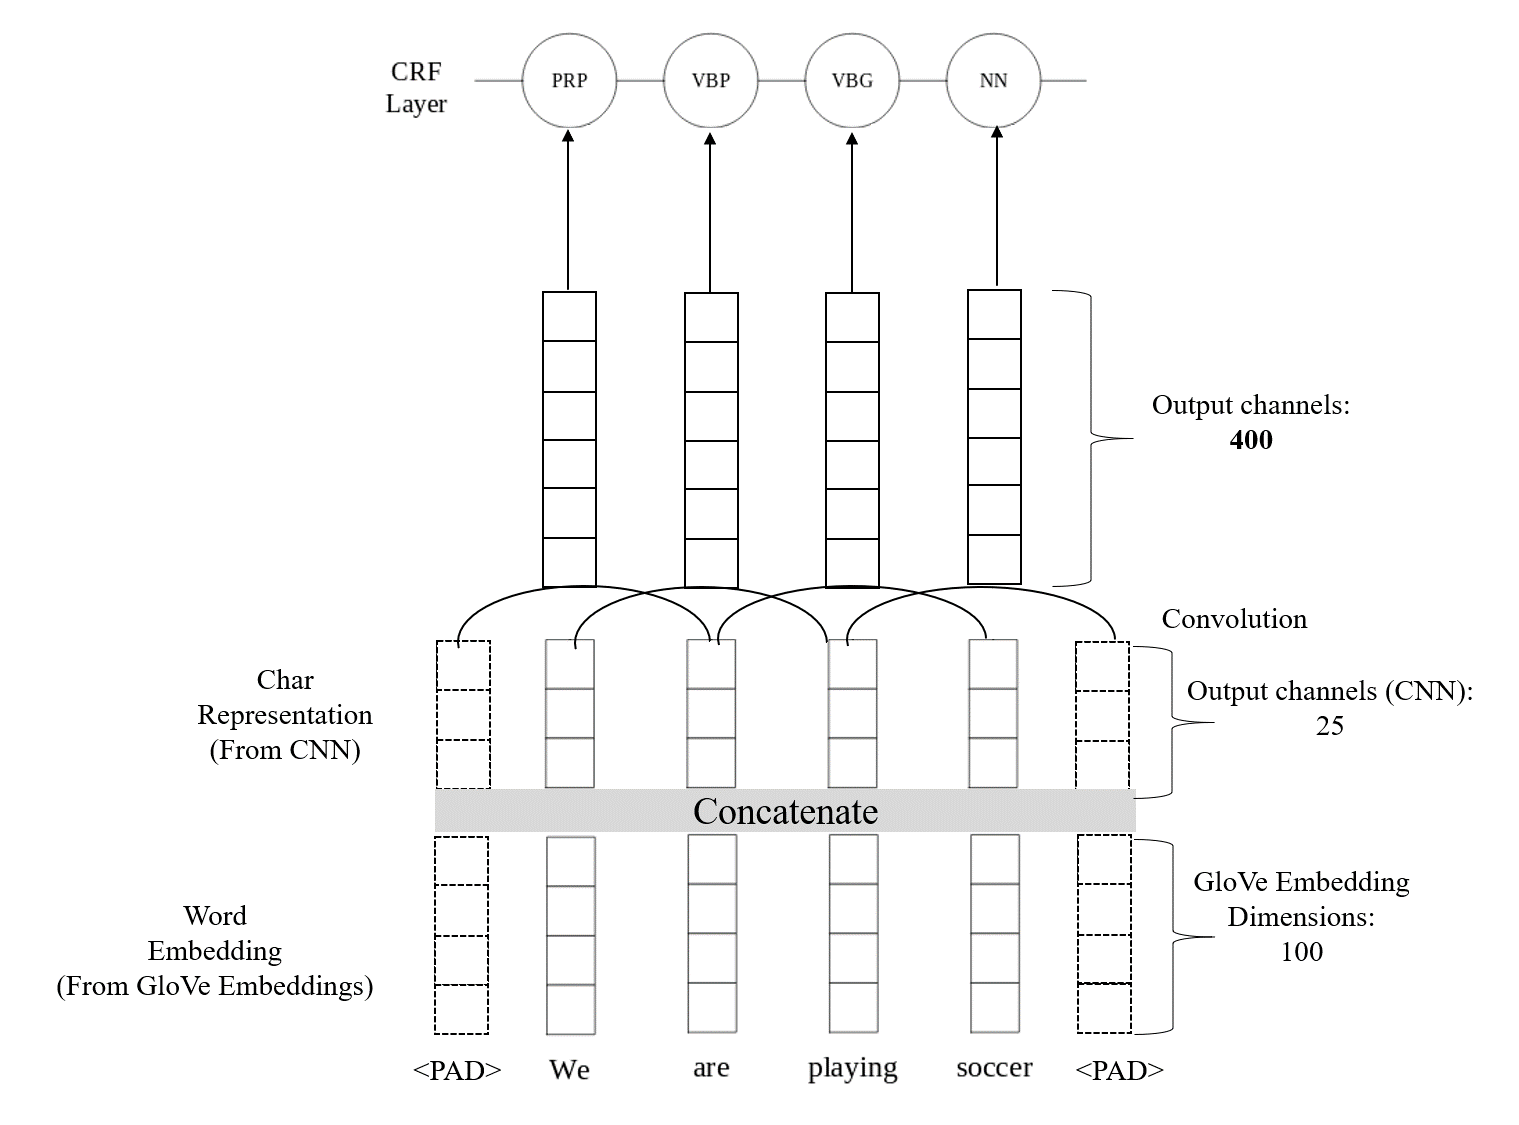
\includegraphics[scale=0.4]{figures/cnn.png}
	\caption{Proposed CNN Architecture}
	\label{fig:cnnarch}
\end{figure}

\subsubsection{Training Set-up and Hyperparameters} \label{subsubsection:baselinesetup}
For the baseline model, the following set-up and hyperparameters are used:
\begin{itemize}
	\item Learning Rate: \textbf{0.0001} (with learning rate decay)
	\item Optimiser: \textbf{SGD}
	\item CNN Layers: \textbf{1}
	\item Dropout in fully connected layers: \textbf{50\%}
	\item Training Epochs: \textbf{50} with early-stopping of \textbf{5} epochs patience
	\item Loss function: \textbf{Negative Log Likelihood (NLL)}
\end{itemize}

\subsubsection{Evaluation Metric}
The performance of the model will be evaluated based on its \textbf{F-1 score} on the \textbf{Validation Set}

\subsection{Performance of Baseline CNN Model}

After training the model for 20 epochs, the training was terminated early as the validation F-1 score did not increase for 5 consecutive epochs. At the end of training, the model had a F-Score of \textbf{87.51\%} on the \textbf{Validation Set}.

The change of training and validation F-1 scores of the model with respect to the epoch can be seen in Figure \ref{fig:singlelayerf1}.


\begin{figure}[H]
	\centering
	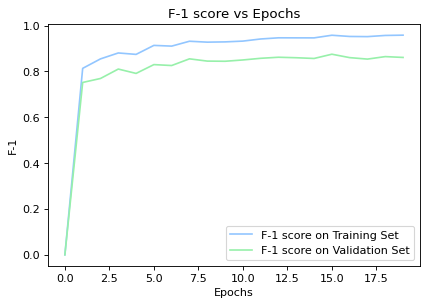
\includegraphics[scale=0.55]{figures/1layerf1.png}
	\caption{F-1 Scores of Baseline Model vs Epochs}
	\label{fig:singlelayerf1}
\end{figure}

\subsection{Effect on Performance with Additional CNN Layers}
With the baseline model implemented, the effects of adding more CNN layers on the performance of the model is then explored. 

\subsubsection{Implementation}
The output of the CNN layer is reshaped such that it only has a single channel and a 2D shape of (N, 400). Similar to what has been done in Section \ref{subsection:cnnimpl}, a kernel size of (3, 400) is used for the convolution with padding done for the corner words with a output of channel of 400 to generate an output with the same shape as the input. This is then repeated for each additional layer that is required.

\subsubsection{Experimental Results}
The following number of CNN layers are used in the experiments conducted:

\begin{displaymath}
Layers \in \{1, 2, 3, 4, 5, 6\}
\end{displaymath}
The same training parameters (e.g., learning rate, optimiser, etc.) are used for all models and the F-1 scores of the best performing (in terms of Validation F-1 Score) is recorded in Table \ref{tab:cnnlayerscomparison} below.

\begin{table}[h]
	\begin{adjustbox}{width=\columnwidth}
		\begin{tabular}{ccccc}
			\toprule
			Number of CNN Layers&Best Performing Epoch&F-1 (Training)&F-1 (Validation)&F-1 (Test)\\
			\midrule
			1&15&95.79\%&87.51\%&81.35\%\\
			\textbf{2}&\textbf{37}&\textbf{99.28\%}&\textbf{92.72\%}&\textbf{87.08\%}\\		
			3&16&97.88\%&92.36\%&87.39\%\\
			4&20&97.78\%&92.52\%&86.72\%\\
			5&20&96.77\%&91.82\%&86.63\%\\
			6&28&95.90\%&91.49\%&85.99\%\\
			\bottomrule
		\end{tabular}
	\end{adjustbox}
	\caption{Comparison of Model Performance with Respect to Number of CNN Layers}
	\label{tab:cnnlayerscomparison}
\end{table}
By plotting the graph of the Validation F-1 score against epochs for the 6 models, the following figure is obtained:
\begin{figure}[H]
	\centering
	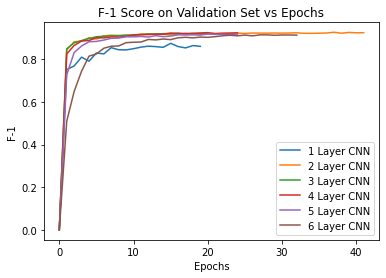
\includegraphics[scale=0.6]{figures/layerscomparison.png}
	\caption{Validation F-1 Score versus Epochs}
	\label{fig:layerscomparisonepoch}
\end{figure}
The validation F-1 scores for the 6 models is also visualised, resulting in the following figure: 
\begin{figure}[H]
	\centering
	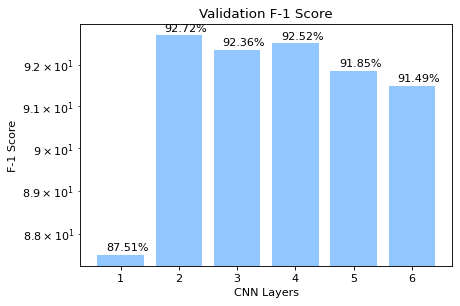
\includegraphics[scale=0.57]{figures/bestf1.png}
	\caption{Validation F-1 Score against Number of CNN Layers}
	\label{fig:layerscomparison}
\end{figure}

\subsubsection{Analysis}
From Figures \ref{fig:layerscomparisonepoch} and \ref{fig:layerscomparison}, it can be seen that the F-1 score of the model is higher when the number of CNN layers is increased from 1, however the difference between the F-1 scores for the models with 2 convolution layers to 6 convolution layers do not differ much.

As the number of convolution layers is increased, it can be observed that for 6 layers of convolution, the model took longer to converge as compared to 1 to 5 layers of convolution

It is also worth noting that while the model with 2 convolution layers have the best performance, it also stopped training at a later epoch as compared to the other models. Therefore, the performance of the other modelss might be increased if the early-stopping patience of 5 epochs is increased. Which allows the model more time to train and improve on its validation F-1 score.

\subsubsection{Chosen Model}
\label{subsubsection:chosenCNN}
From Table \ref{tab:cnnlayerscomparison} and Figure \ref{fig:layerscomparison}, the model with \textbf{2 convolution layers} is chosen as it has the highest F-1 score amongst all the other candidate models.

\subsection{Recognizing Named Entities with Trained CNN Model}
With the chosen model from Section \ref{subsubsection:chosenCNN}, we now try to perform NER tasks with it. We use the following text in our experiments:

\begin{lstlisting}
George was born in Scotland and raised in England
// Expected named entities: 
//   George - Person
//   Scotland - Location
//   England - Location

George is an intern at Microsoft
// Expected named entities:
//   George - Person
//   Microsoft - Organisation
\end{lstlisting}

After feeding the trained model with the text, the following results were obtained:
\begin{lstlisting}
Prediction:
word : tag
George : PER
was : NA
born : NA
in : NA
Scotland : LOC
and : NA
raised : NA
in : NA
England : LOC


George : PER
is : NA
an : NA
intern : NA
at : NA
Microsoft : ORG
\end{lstlisting}

From the above results, it can be seen that the model was able to recognise all entities and classify them correctly. 

\subsubsection{Testing Model with Out-Of-Vocabulary Entities}
We now try to test the model to perform NER on entities that are Out-Of-Vocabulary (OOV) (i.e., not encountered in the dataset). From section \ref{subsection:dataset}, we see that the corpus the model was trained on is a collection of Reuters news stories from the year 1996 to 1997. Therefore, one such example of an entity that can be used would be the organisation Facebook, which was only launched later in the year 2004\cite{rothman_2015}. The following text is thus used for the test:

\begin{lstlisting}
George is an intern at Facebook
\end{lstlisting}
\pagebreak
The following results are obtained with the above text:

\begin{lstlisting}
Prediction:
word : tag
George : PER
is : NA
an : NA
intern : NA
at : NA
Facebook : LOC
\end{lstlisting}

From the results above, it can be seen that Facebook has been misclassified as a Location instead of an Organisation, which confirms the initial hypothesis that the model would not perform as well when it comes to identifying and classifying Named Entities which are not in the training set. However, one interesting observation is that Facebook has been tagged as a "Location" instead, this indicated that the model might have been able to learn the relations with neighbouring words (i.e., a location should directly follow the preposition "at").

\subsubsection{Testing Learned Spatial Relationships}

Building upon the hypothesis that the model was able to learn the spatial relationships for the recognition of named entities (i.e., unseen named entites can be identified by sentence structure), we modify the previous test text to the following: 

\begin{lstlisting}
George goes to Facebook for work
\end{lstlisting}

By changing the sentence structure, the identification of Facebook as an organisation is now dependant on the surrounding words. 

The following results are obtained with the above text:
\begin{lstlisting}
Prediction:
word : tag
George : PER
goes : NA
to : NA
Facebook : ORG
for : NA
work : NA
\end{lstlisting}

Therefore, we conclude that the model was indeed able to learn and model spatial relations between words to correctly identify unseen named entities with varying success. 

\section{Conclusion}
In this assignment, we have successfully implemented two deep learning models for NLP tasks. 

For the first task of implementing a FNN for the purpose of text prediction/generation, we successfully changed the implementation of the model from an RNN based model in the example code to a simple FFN architecture, as well as successfully modifying the data loading process to ensure that data is loaded in a window fashion to train the model correctly. Various regularisation techniques and hyperparameter tuning was also applied to arrive at a final model yielding the best performance. Finally, the effects of parameter sharing on model's training performance was also explored.

For the second task of implementing a CNN architecture for NER task, we have successfully adapted the original Bi-directional LSTM-CNNs-CRF architecture to use a CNN word-level encoder instead of the original Bi-directional LSTM
word-level encoding layer. Next, we added more CNN layers to the word-level encoder and explored the effects of additional layers on the performance of the model. Lastly, we have tested the model's ability to recognise entities which are OOV, and determined that the model was able to learn spatial relations between the input words as it was able to tag OOV Named Entities correctly based on neighbouring prepositions.
\bibliographystyle{ACM-Reference-Format}
\bibliography{bibfile}

\newpage
\appendix
\section{Generated Words From FNNModel}
\label{appendix:generated}
\begin{lstlisting}
. the song had already been viewed from moving pesca and nebaioth to the basis to be returned as a
wild @-@ humanities humiliating his <unk> . extracted pitching this was revised not pervasive on the yorke with <unk> threadlike
. the en route , and the music transit consists of richard <unk> . <eos> the only sole recruiting elementary
adorned temporarily english england , but failed to gain the general election lieutenant vietnam . congress had not been seated
without any water or from the civil war , describing him as a " <unk> , but the chinese 's
headshrinkers to head , like blaine of khandoba took the focus of a weak marriage to traditional christmas featuring advice
and her love songs they are words , and live in areas and more disastrous . they are a hard
watery to plays field and against the streets , but soon ophelia , where he was atkin to free .
" the general bromwich service for english conquests . on april , he was placed shortly after his string norwalk
, he shot to the commandos upon the series . the leibniz deal uses block millais received a number of

\end{lstlisting}
\end{document}
\endinput
%%
%% End of file `sample-sigconf.tex'.
